\documentclass[12pt, titlepage]{article}
\usepackage[table]{xcolor} 
\usepackage{colortbl} 
\usepackage{geometry} 
\usepackage{caption}
\usepackage{array} 
\usepackage{booktabs}
\usepackage{multirow}
\usepackage{booktabs}
\usepackage{tabularx}
\usepackage{graphicx}
\usepackage{float}
\usepackage{hyperref}
\hypersetup{
    colorlinks,
    citecolor=black,
    filecolor=black,
    linkcolor=red,
    urlcolor=blue
}
\usepackage[round]{natbib}

%% Comments

\usepackage{color}

\newif\ifcomments\commentstrue %displays comments
%\newif\ifcomments\commentsfalse %so that comments do not display

\ifcomments
\newcommand{\authornote}[3]{\textcolor{#1}{[#3 ---#2]}}
\newcommand{\todo}[1]{\textcolor{red}{[TODO: #1]}}
\else
\newcommand{\authornote}[3]{}
\newcommand{\todo}[1]{}
\fi

\newcommand{\wss}[1]{\authornote{blue}{SS}{#1}} 
\newcommand{\plt}[1]{\authornote{magenta}{TPLT}{#1}} %For explanation of the template
\newcommand{\an}[1]{\authornote{cyan}{Author}{#1}}

%% Common Parts

\newcommand{\progname}{Course Buddy} % PUT YOUR PROGRAM NAME HERE
\newcommand{\authname}{Team \#5, Overwatch League
\\ Jingyao, Qin
\\ Qianni, Wang
\\ Qiang, Gao
\\ Chenwei, Song
\\ Shuting, Shi
\\ } % AUTHOR NAMES                  

\usepackage{hyperref}
    \hypersetup{colorlinks=true, linkcolor=blue, citecolor=blue, filecolor=blue,
                urlcolor=blue, unicode=false}
    \urlstyle{same}
                                


\begin{document}

\title{Verification and Validation Report: \progname} 
\author{\authname}
\date{\today}
	
\maketitle

\pagenumbering{roman}

\section{Revision History}

\begin{tabularx}{\textwidth}{p{3cm}p{2cm}X}
\toprule {\bf Date} & {\bf Version} & {\bf Notes}\\
\midrule
2024-03-06 & 1.0 & -\\
\bottomrule
\end{tabularx}

~\newpage

\section{Symbols, Abbreviations and Acronyms}

\renewcommand{\arraystretch}{1.2}
\begin{tabular}{l l} 
  \toprule		
  \textbf{symbol} & \textbf{description}\\
  \midrule 
      UI & User Interface \\
      API & Application Programming Interface\\
      HTTP & Hypertext Transfer Protocol\\
      PDF & Portable Document Format\\
      .csv & Comma-Separated Values \\
      .txt & Text file\\
  \bottomrule
  
\end{tabular}\\
\newpage

\tableofcontents

\listoftables %if appropriate

\listoffigures %if appropriate

\newpage

\pagenumbering{arabic}


\section{Functional Requirements Evaluation}
\subsection{Unit Testing}
\subsubsection{test\_download}\label{3.1.1}
\begin{itemize}
    \item Description: Testing download outline functionality
    \item Requirement Reference: To be updated
    \item Inputs: Request file `testfile.txt` 
    \item Expected Outputs: File content in response.data  
    \item Actual Outputs: File content in response.data  
    \item Result: Pass
\end{itemize}
\subsubsection{test\_change\_username}\label{3.1.2}
\begin{itemize}
    \item Description: Testing username change
    \item Requirement Reference: To be updated
    \item Inputs: New username `new\_user`
    \item Expected Outputs: Updated username `new\_user` in response.data
    \item Actual Outputs: Updated username `new\_user` in response.data
    \item Result: Pass
\end{itemize}
\subsubsection{test\_remove\_course}\label{3.1.3}
\begin{itemize}
    \item Description: Testing course removal
    \item Requirement Reference: To be updated
    \item Inputs: Index of course to remove
    \item Expected Outputs: Course list without the course
    \item Actual Outputs: Course list without the course
    \item Result: Pass
\end{itemize}
\subsubsection{test\_course\_detail}\label{3.1.4}
\begin{itemize}
    \item Description: Testing course detail retrieval
    \item Requirement Reference: FR15
    \item Inputs: Course ID `4C03`
    \item Expected Outputs: Course details page containing Course ID `4C03`
    \item Actual Outputs: Course details page containing Course ID `4C03`
    \item Result: Pass
\end{itemize}
\subsubsection{test\_upload\_file}\label{3.1.5}
\begin{itemize}
    \item Description: Testing file upload
    \item Requirement Reference: FR5
    \item Inputs: File `test.pdf`
    \item Expected Outputs: Success message "File uploaded successfully!"
    \item Actual Outputs: Success message "File uploaded successfully!"
    \item Result: Pass
\end{itemize}
\subsubsection{test\_add\_course}\label{3.1.6}
\begin{itemize}
    \item Description: Testing addition of new course
    \item Requirement Reference: FR5
    \item Inputs: New course `new\_course`
    \item Expected Outputs: `new\_course` in response.data
    \item Actual Outputs: `new\_course` in response.data
    \item Result: Pass
\end{itemize}
\subsubsection{test\_course\_page}\label{3.1.7}
\begin{itemize}
    \item Description: Testing course page display
    \item Requirement Reference: To be updated
    \item Inputs: None
    \item Expected Outputs: ["course1", "course2"] in response.data
    \item Actual Outputs: ["course1", "course2"] in response.data
    \item Result: Pass
\end{itemize}
\subsubsection{test\_profile\_page}\label{3.1.8}
\begin{itemize}
    \item Description: Testing profile page display
    \item Requirement Reference: To be updated
    \item Inputs: None
    \item Expected Outputs: "/change\_username" in response.data
    \item Actual Outputs: "/change\_username" in response.data
    \item Result: Pass
\end{itemize}
\subsubsection{test\_feedback\_page}\label{3.1.9}
\begin{itemize}
    \item Description: Testing feedback page access
    \item Requirement Reference: To be updated
    \item Inputs: None
    \item Expected Outputs: "Submit Feedback" in response.data
    \item Actual Outputs: "Submit Feedback" in response.data
    \item Result: Pass
\end{itemize}
\subsubsection{test\_submit\_feedback}\label{3.1.10}
\begin{itemize}
    \item Description: Testing feedback submission
    \item Requirement Reference: To be updated
    \item Inputs: feedback\_data = \{
        "name": "John Doe",
        "email": "john.doe@example.com",
        "feedback\_type": "General",
        "feedback": "Great app!"
    \}
    \item Expected Outputs: Redirect to the feedback page
    \item Actual Outputs: Redirect to the feedback page
    \item Result: Pass
\end{itemize}
\subsubsection{test\_forum\_page}\label{3.1.11}
\begin{itemize}
    \item Description: Testing forum page access
    \item Requirement Reference: To be updated
    \item Inputs: None
    \item Expected Outputs: "MacForum - The McMaster community discussion board" in response.data
    \item Actual Outputs: "MacForum - The McMaster community discussion board" in response.data
    \item Result: Pass
\end{itemize}
\subsubsection{test\_add\_topic}\label{3.1.12}
\begin{itemize}
    \item Description: Testing topic addition in forum 
    \item Requirement Reference: To be updated
    \item Inputs: topic\_data = \{
        "title": "Test Topic",
        "description": "This is a test topic description.",
    \}
    \item Expected Outputs: topic\_data in response.data
    \item Actual Outputs: topic\_data in response.data
    \item Result: Pass
\end{itemize}
\subsubsection{test\_topic}\label{3.1.13}
\begin{itemize}
    \item Description: Testing topic page access in the forum
    \item Requirement Reference: To be updated
    \item Inputs: Topic ID `1`  
    \item Expected Outputs: "Best Study Spots on Campus" in response.data
    \item Actual Outputs: "Best Study Spots on Campus" in response.data
    \item Result: Pass
\end{itemize}

\subsubsection{test\_upload\_transcript}\label{3.1.14}
\begin{itemize}
    \item Description: Testing transcript upload
    \item Requirement Reference: To be updated
    \item Inputs: File "transcript.pdf"
    \item Expected Outputs: "Profile Page" in response.data
    \item Actual Outputs: "Profile Page" in response.data
    \item Result: Pass
\end{itemize}
\subsubsection{test\_upload\_transcript\_processing}\label{3.1.15}
\begin{itemize}
    \item Description: Testing transcript cGPA processing after upload
    \item Requirement Reference: To be updated
    \item Inputs: File "transcript.pdf"
    \item Expected Outputs: "9.4/12" in response.data
    \item Actual Outputs: "9.4/12" in response.data
    \item Result: Pass
\end{itemize}
\subsubsection{test\_delete\_task}\label{3.1.16}
\begin{itemize}
    \item Description: Testing task deletion 
    \item Requirement Reference: To be updated
    \item Inputs:  "id": [
                task\_id,
                2,
            ], 
    \item Expected Outputs: task\_id not in response.data
    \item Actual Outputs: task\_id not in response.data
    \item Result: Pass
\end{itemize}

\subsubsection{test\_edit\_task}\label{3.1.17}
\begin{itemize}
    \item Description: Testing task editing 
    \item Requirement Reference: To be updated
    \item Inputs:  task\_data = \{
        "task\_name": "Updated Task",
        "due\_date": "2021-01-01",
        "weight": "5",
        "est\_hours": "2",
    \}
    \item Expected Outputs: task\_data in response.data
    \item Actual Outputs: task\_data in response.data
    \item Result: Pass
\end{itemize}


\subsection{Manual Testing}
\subsubsection{TFR1\_A1}\label{3.2.1}
\begin{itemize}
    \item Description: Change Testing username change
    \item Requirement Reference: To be updated
    \item Inputs: The user navigates to the profile page, enters "newName" in the "change username" input field, clicks the "Submit" button
    \item Expected Outputs: Redirect to the home page with "Hello, newName! Welcome to Mac One!"
    \item Actual Outputs: Redirect to the home page with "Hello, newName! Welcome to Mac One!"
    \item Result: Pass
\end{itemize}

\subsubsection{TFR2-UI1}\label{3.2.2}
\begin{itemize}
    \item Description: Submit feedback
    \item Requirement Reference: To be updated
    \item VnV Plan Reference: To be updated
    \item Inputs: The user navigates to the feedback page, fills the form, clicks the "Submit Feedback" button
    \item Expected Outputs: Success message "Thank you for your feedback!"
    \item Actual Outputs: Success message "Thank you for your feedback!"
    \item Result: Pass
\end{itemize}

\subsubsection{TFR3-UI1}\label{3.2.3}
\begin{itemize}
    \item Description: Add a topic
    \item Requirement Reference: To be updated
    \item VnV Plan Reference: To be updated
    \item Inputs: The user navigates to the forum page, clicks "Add Topic" button, fills the form, clicks the "Submit" button
    \item Expected Outputs: Redirects the forum page with the new topic listed.
    \item Actual Outputs: Redirects the forum page with the new topic listed.
    \item Result: Pass
\end{itemize}

\subsubsection{TFR3-UI2}\label{3.2.4}
\begin{itemize}
    \item Description: Add a Comment
    \item Requirement Reference: To be updated
    \item VnV Plan Reference: To be updated
    \item Inputs: The user navigates to the forum page, clicks a topic, fills the comment input field, clicks the "Submit" button
    \item Expected Outputs: The new comment is listed under the selected topic.
    \item Actual Outputs: The new comment is listed under the selected topic.
    \item Result: Pass
\end{itemize}

\subsubsection{TFR3-UI3}\label{3.2.5}
\begin{itemize}
    \item Description: Add a Comment
    \item Requirement Reference: To be updated
    \item VnV Plan Reference: To be updated
    \item Inputs: The user navigates to the forum page, inputs keywords in the search box, click the "Search" button
    \item Expected Outputs: Lists of topics and comments containing the searched keywords are displayed.
    \item Actual Outputs: Lists of topics and comments containing the searched keywords are displayed.
    \item Result: Pass
\end{itemize}

\subsubsection{TFR4-UI1}\label{3.2.6}
\begin{itemize}
    \item Description: Get cGPA
    \item Requirement Reference: To be updated
    \item VnV Plan Reference: To be updated
    \item Inputs: The user navigates to the profile page, chooses a local transcript PDF file, and clicks the "Upload Transcript" button.
    \item Expected Outputs: The cGPA calculated is displayed.
    \item Actual Outputs: The cGPA calculated is displayed.
    \item Result: Pass
\end{itemize}


\subsubsection{TFR6-UI1}\label{3.2.7}
\begin{itemize}
    \item Description: Upload PDF
    \item Requirement Reference: To be updated
    \item VnV Plan Reference: TFR6-UI1
    \item Inputs: The user navigates to a course page, selects a local course outline, clicks the "Upload File" button
    \item Expected Outputs: Success message "File uploaded successfully!"
    \item Actual Outputs: Success message "File uploaded successfully!"
    \item Result: Pass
\end{itemize}

\subsubsection{TFR6-UI2}\label{3.2.8}
\begin{itemize}
    \item Description: Update task progress
    \item Requirement Reference: FR13
    \item VnV Plan Reference: TFR6-UI12
    \item Inputs: The user navigates to the homepage, clicks and drags one of the tasks to another progress zone.
    \item Expected Outputs: The task stays at the new zone.
    \item Actual Outputs: The task stays at the new zone.
    \item Result: Pass
\end{itemize}

\subsubsection{TFR6-UI3}\label{3.2.9}
\begin{itemize}
    \item Description: Delete task
    \item Requirement Reference: To be updated
    \item VnV Plan Reference: To be updated
    \item Inputs: The user navigates to the homepage, and clicks the delete button of a selected task.
    \item Expected Outputs: The task disappears.
    \item Actual Outputs: The task disappears.
    \item Result: Pass
\end{itemize}

\subsubsection{TFR9-UI1}\label{3.2.10}
\begin{itemize}
    \item Description: Start a Pomodoro timer
    \item Requirement Reference: FR29
    \item VnV Plan Reference: To be updated
    \item Inputs: The user navigates to the Pomodoro page, and clicks the "Start" button.
    \item Expected Outputs: The Pomodoro countdown starts.  A tomato icon is added when the countdown reaches zero.
    \item Actual Outputs: The Pomodoro countdown starts.  A tomato icon is added when the countdown reaches zero.
    \item Result: Pass
\end{itemize}

\subsubsection{TFR9-UI2}\label{3.2.11}
\begin{itemize}
    \item Description: Reset a Pomodoro timer
    \item Requirement Reference: FR29
    \item VnV Plan Reference: To be updated
    \item Inputs: The user navigates to the Pomodoro page, and clicks the "Start" button, and clicks the "Reset" button before the countdown finishes.
    \item Expected Outputs: The Pomodoro countdown resets to the default.
    \item Actual Outputs: The Pomodoro countdown resets to the default.
    \item Result: Pass
\end{itemize}

\subsubsection{TFR9-UI3}\label{3.2.12}
\begin{itemize}
    \item Description: Play music.
    \item Requirement Reference: To be updated
    \item VnV Plan Reference: To be updated
    \item Inputs: The user navigates to the Pomodoro page, and clicks the "Play Music" button.
    \item Expected Outputs: Music is played.
    \item Actual Outputs: Music is played.
    \item Result: Pass
\end{itemize}

\subsubsection{TFR9-UI4}\label{3.2.13}
\begin{itemize}
    \item Description: Play music.
    \item Requirement Reference: To be updated
    \item VnV Plan Reference: To be updated
    \item Inputs: The user navigates to the Pomodoro page, selects another genre from the drop-down menu, and clicks the "Play Music" button.
    \item Expected Outputs: Selected music is played.
    \item Actual Outputs: Selected music is played.
    \item Result: Pass
\end{itemize}



\subsubsection{TFR16-17-D1}\label{3.2.14}
\begin{itemize}
    \item Description: Extract data from PDF
    \item Requirement Reference: FR15
    \item VnV Plan Reference: TFR16-17-D1
    \item Inputs: The user presses to extract the course information from the uploaded
PDF
    \item Expected Outputs: The page shows lists of the course information extracted from the PDF
as a task list
    \item Actual Outputs: The page shows lists of the course information extracted from the PDF
as a task list
    \item Result: Pass
\end{itemize}

\subsubsection{TFR21-D5}\label{3.2.15}
\begin{itemize}
    \item Description: Tasks display
    \item Requirement Reference: FR16
    \item VnV Plan Reference: TFR21-D5
    \item Inputs: The start and end times of the working hours for certain tasks recorded
by using the Pomodoro Timmers, the estimated progress user input at
the end of the Pomodoro Timmers, as well as the user’s list of tasks and the
percentage of progress of the marked tasks.
    \item Expected Outputs: Displays to the user a list of tasks with status labels.
    \item Actual Outputs: Displays to the user a list of tasks with status labels.
    \item Result: Pass
\end{itemize}


\subsubsection{TFR26-S2}\label{3.2.16}
\begin{itemize}
    \item Description: Tasks information update
    \item Requirement Reference: FR26
    \item VnV Plan Reference: TFR26-S2
    \item Inputs: Current schedule data for the task includes deadline, priority, weight,
current progress in completing the task, the user’s history of the percentage of
progress completed, and the corresponding time spent on the task.
    \item Expected Outputs: The updated Learning Plan, regenerated task schedule information
based on the updated task progress from the user, which may include reordering
of task list and TO-DO list, new priority of the task, etc.
    \item Actual Outputs: The updated Learning Plan, regenerated task schedule information
based on the updated task progress from the user, which may include reordering
of task list and TO-DO list, new priority of the task, etc.
    \item Result: Pass
\end{itemize}

\subsubsection{TFR28-S4}\label{3.2.17}
\begin{itemize}
    \item Description: Tasks ranking
    \item Requirement Reference: TFR28
    \item VnV Plan Reference: TFR28-S4
    \item Inputs: The user’s task list and data for tasks including taskType, weight and
deadline.
    \item Expected Outputs: A task priority list, based on sorting the tasks in order by task type,
weight, and deadline. High-priority tasks will be ranked first.
    \item Actual Outputs: A task priority list, based on sorting the tasks in order by task type,
weight, and deadline. High-priority tasks will be ranked first.
    \item Result: Pass
\end{itemize}



\section{Nonfunctional Requirements Evaluation}

\subsection{Usability}
\subsubsection{Survey}\label{4.1.1}
\textbf{Testing Progress} \\

\noindent A usability testing survey was completed by 10 participants, all of whom are students, with 8 attending McMaster University. Participants were invited to provide their feedback through a Google Forms survey, with the questions outlined in Section 6.2 of the Verification and Validation (VnV) plan.\\

\noindent \textbf{Result}
\begin{table}[htb!]
\caption{Survey Result for Usability}
\begin{tabular}{|l|c|}
\hline
\textbf{Survey Result for Usability}                                                                                                    & \textbf{Result Value} \\ \hline
\begin{tabular}[c]{@{}l@{}}Percentage of users who found the content of the website \\ clear and easy to understand\end{tabular}             & 78\%                  \\ \hline
\begin{tabular}[c]{@{}l@{}}Average percentage score of user feedback on overall ease\\ of use of site navigation\end{tabular}                & 62\%                  \\ \hline
\begin{tabular}[c]{@{}l@{}}Average percentage score of user feedback on ease of use \\ of the prioritization generation feature\end{tabular} & 28\%                  \\ \hline
\end{tabular}
\end{table}

\noindent \textbf{Analysis} \\

\noindent The result of the survey indicates that the current level of clarity, ease of use, and understanding of our website does not meet the predefined minimum threshold outlined in our Validation and Verification (VnV) plan (90\%). This outcome underscores a significant need for enhancement in several key areas to elevate the overall user experience, for example, improving our UI elements, adding new features and simplifying processes to perform certain tasks.

\subsubsection{Observation Study}\label{4.1.2}

\textbf{Testing Process} \\

\noindent To understand user interactions with our website, we conducted an observation study that involved 10 students from McMaster University, selected for their diverse backgrounds and familiarity with similar digital interfaces. The primary objective was to closely monitor and analyze their overall user experience while engaging with specific, predetermined tasks. These tasks were designed to mimic common user cases such as navigating to designated pages within our website. Two of our developers were assigned to perform the study and conduct the observations. Each participant's approach to the tasks, including the ability to perform specific tasks, interaction with UI elements, and additional comments, was documented.\\

\noindent \textbf{Result}\\

\noindent The result of the test is shown in the table below:
\clearpage
\begin{table}[htb!]
\footnotesize
\caption{Observation Result for Usability}
\begin{tabular}{|l|l|c|c|c|}
\hline
\textbf{Test Plan} & \textbf{How test has been performed}                                                                                                                                                                                                       & \textbf{Actual Result} & \multicolumn{1}{l|}{\textbf{Expected Result}} & \multicolumn{1}{l|}{\textbf{Result}} \\ \hline
THUR-1   \label{THUR-1 }          & \begin{tabular}[c]{@{}l@{}}Users are asked to navigate to a \\ required page, the result \\ of the percentage of users who \\ are able to navigate to the \\ page without confusion are\\ calculated.\end{tabular}                           & 60\%                  & 90\%                                          & Fail                                 \\ \hline
THUR-2    \label{THUR-2 }          & \begin{tabular}[c]{@{}l@{}}Ask users to upload a course \\ syllabus file and calculate the \\ percentage of users who are able \\ to use this feature without \\ problems.\end{tabular}                                                    & 70\%                    & 90\%                                          & Fail                                 \\ \hline
THUR-2             & \begin{tabular}[c]{@{}l@{}}Ask users to generate the priority \\ of a course work by using \\ the priority prediction model and \\ calculate the percentage of \\ users who are able to use this \\ feature without problems.\end{tabular} & 40\%                    & 90\%                                          & Fail                                 \\ \hline
THUR-2             & \begin{tabular}[c]{@{}l@{}}Ask users to change the user name \\ in the website and calculate \\ the percentage of users who \\ are able to use this feature \\ without problems.\end{tabular}                                              & 100\%                   & 90\%                                          & Pass                                 \\ \hline
THUR-3     \label{THUR-3 }        & \begin{tabular}[c]{@{}l@{}}Ask users to check the grammar \\ of text on a page. Calculate \\ the average number of grammatical \\ errors found by the user.\end{tabular}                                                                   & 1.5                   & 0                                             & Fail                                 \\ \hline
THUR-4    \label{THUR-4 }         & \begin{tabular}[c]{@{}l@{}}Ask users to check if there is \\ any offisive message in the \\ website. Calculate the average \\ number of offiensive messages \\ found by the user.\end{tabular}                                             & 0                     & 0                                             & Pass                                 \\ \hline
THUR-5    \label{THUR-5 }         & \begin{tabular}[c]{@{}l@{}}Ask users to observe the color \\ combinations on the page. \\ Count the number of areas of \\ the site's user interface \\ where users find color combinations \\ difficult to distinguish.\end{tabular}       & 3                     & 0                                             & Fail                                 \\ \hline
\end{tabular}
\end{table}
\clearpage

\noindent \textbf{Analysis}

\noindent The result reveals that the proportion of users who successfully navigate to certain pages or complete specific tasks falls below our expected value of 90\%, as outlined in Section 6.2 of our Verification and Validation (VnV) plan. This discrepancy highlights the necessity for modifications to enhance user navigation and task execution. Accordingly, improvements in the user interface, particularly the navigation bar, and the simplification of task processes are needed. Additionally, we need to address some small grammar mistakes for a better and smoother user experience as on average there are 1.5 grammar mistakes found.


\subsection{Accuracy}
\subsubsection{Manual Testing}

\textbf{Testing Process} \\

\noindent To ensure the accuracy of our main feature that extracts course information from PDF outlines, we conducted manual testing. For this purpose, two members of our development team chose five different course outlines which were randomly to represent a variety of courses. Each selected course outline was then uploaded to our website to start the course information extraction process.
After the extraction was complete for each outline, our developers manually examined the results on the website closely. They checked if the course information such as course codes, and descriptions was accurately extracted. Then they calculated and recorded how much of the information was correctly extracted from each course outline.
\clearpage
\noindent \textbf{Result}
\begin{itemize}
    \item Extract course information using the regular method.
    \begin{table}[htb!]
    \caption{Manual Testing Regular Expression Method for Accuracy}
    \footnotesize
    \begin{tabular}{|l|l|c|c|c|}
    \hline
    \textbf{Test Plan} & \textbf{How test has been performed}                                                                                                                                                                                                       & \textbf{Actual Result} & \multicolumn{1}{l|}{\textbf{Expected Result}} & \multicolumn{1}{l|}{\textbf{Result}} \\ \hline
    TPAR-1             & \begin{tabular}[c]{@{}l@{}}Manually upload multiple course \\syllabus documents and record the \\percentage of course information \\correctly extracted.\end{tabular}                           & 23.6\%                  & 90\%                                          & Fail                                 \\ \hline
    \end{tabular}
    \end{table}
    \item{Extract course information using OpenAI API.}\
    \begin{table}[htb!]
    \caption{Manual Testing OpenAI API Method for Accuracy}
    \footnotesize
    \begin{tabular}{|l|l|c|c|c|}
    \hline
    \textbf{Test Plan} & \textbf{How test has been performed}                                                                                                                                                                                                       & \textbf{Actual Result} & \multicolumn{1}{l|}{\textbf{Expected Result}} & \multicolumn{1}{l|}{\textbf{Result}} \\ \hline
    TPAR-1             & \begin{tabular}[c]{@{}l@{}}Manually upload multiple course \\syllabus documents and record the \\percentage of course information \\correctly extracted.\end{tabular}                           & 95.6\%                  & 90\%                                          & Pass                                 \\ \hline
    \end{tabular}
    \end{table}

\end{itemize}

\noindent \textbf{Analysis}\\

\noindent As can be seen from the results, the precision of the results obtained using the regular expression method to extract course information from PDF course syllabi is very low and does not meet the minimum precision threshold (90\%) specified in Section 6.1 of the VnV Plan. This indicates that we need to improve the accuracy of the algorithm. Since the accuracy (23.6\%) is well below the threshold, this means that we may need to propose a new algorithm instead of improving the existing one, which would improve the accuracy to a great extent.
We then decided to extract the course information through the OpenAI API by inputting the course syllabus PDF file and collating and extracting the content returned by the API, and the evaluation results showed a significant improvement in the accuracy of extracting the course information using this method, and based on the minimum accuracy threshold of 90\% set out in the Verification and Validation (VnV) Plan, Section 6.1, we can tell that the results of the test (95.6\%) has been passed.

\section{Changes Due to Testing}
% \clearpage
\begin{figure}[H]
    \centering
    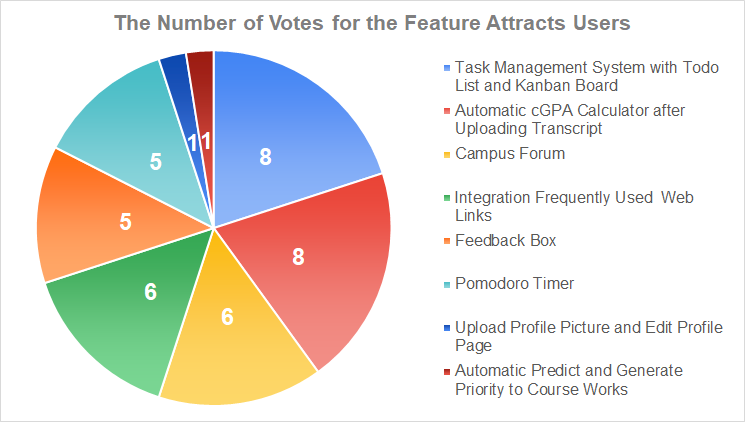
\includegraphics[width=1\linewidth]{VnV/Frequency of use of functions.png}
    \caption{The Number of Votes Got from Survey for Which Feature Attracts Users More}
    \label{fig:enter-label}
\end{figure}




\subsection{Removing Task Priority Prediction Feature}\label{TPPD}
From the result of the survey shown in the Figure 1, we can see that only 1 out of 10 users think that the task priority prediction was attractive. Besides, our initial design of task priority prediction's choice of model requires the high demand of dataset as input to ensure the accuracy of this model. However, in the current stage, it is hard to collect the need amount of data for our model training and make this feature complete and effective. Therefore, we abandoned this feature and put our efforts into other features that are more useful, feasible, and less time-consuming.


\subsection{Changing Algorithm of Course Information Extraction}\label{CIEN}
From the manual testing data result, we can see that there is an urgent need to improve the accuracy of the algorithm so that the percentage of the course information such as course code, and assignment weights that are correctly extracted can be improved. Our original design was simply using Regular Expression to parse each information, however, due to the inconsistency of the format of the course outlines, it is difficult to correctly come up with the Regex pattern to extract related information from various course outlines. Therefore, we decided to use a completely new approach which is to use OpenAI API to parse related course information for us and then we can parse the response sent by the OpenAI server. In this way, our accuracy improves dramatically but our performance suffers a bit as it takes longer to complete the extraction due to the way how OpenAI handles those API calls.


\subsection{Adding Frequently Used Apps Quick Links Feature}\label{IAQL}
From our survey and additional comments when conducting the observational study, we can see that most users think it would be nice to have a feature where users can navigate quick links to key university websites as well as useful study tools that are being used daily such as Microsoft Teams, GitHub, etc. We wanted to improve our user experience as well as continuously improve our website by gathering feedback from users and developing new useful features, therefore we added this useful feature after the testing.

\subsection{Adding Feedback Box Feature}\label{FEEP}

After the testing, we noticed the importance of having continuous improvement and direct user input into our website management and improvement.
We therefore added a feature where we implemented a direct communication method through the feedback box page which allows students to provide our developers with their suggestions directly.  In this kind of sustainable feedback-improving mechanism, we could o continuously improve our website and meet students’ needs as much as possible.

\subsection{Adding cGPA Calculator Feature}\label{PEDC}

According to the results of the votes for the feature attract users, we noticed that most of the users have a high preference for the automatic cGPA calculator after uploading the transcript. Also, the cGPA calculation feature is a very useful tool and a brand-new feature which could not be easily accessed from other resources. Therefore, we decided to add this feature for students to evaluate their study performance, view their academic progress, and make a responsive study plan to improve themselves, which meet our users' needs and satisfaction.

\subsection{Adding Pomodoro \& Weekly achievements Feature}\label{PWAC}

After the testing, we noticed that the pomodoro timer feature is one of the most popular features. Also, even we have transferred our design focus from the study application into a comprehensive McMaster application, we still would like to retain some features that could support students to be able to access efficient study environments and tools. Therefore, This is a feature that aims to help the user have a deeper focus in the virtual study room which could help students manage distraction and control, and decrease back pain and mental fatigue. Also, with the concern of Rev 0 Demo feedback, we should integrate task management with the pomodoro timer. After integration, the user could click the task on the To-Do list board and redirect to the pomodoro timer page with the timer set up according to the task's estimated finish time, which could then massively increase the user’s motivation to study, and highly increase the whole project's user experience.

\subsection{Adding Forum Discussion Board Feature}\label{FDBD}

 Campus forum has been presented as the top four attractive features in the user-survey. The forum allows users to easily search the topics they are interested in and comment on the existing topic to quickly get involved in. Also, this feature supports users to create new topics enabling students to initiate the discussion they would like to arise. Therefore, the students could participate in an inclusive,  interactive, and collaborative community and obtain the information they would like to know. 
 
\subsection{Improving the main UI elements}\label{IMUI}
From the testing result and analysis, we can see that we need to improve our UI elements such as the layout of the navigation bar and overall user interface to enhance usability. Therefore, we redesigned our navigation bar to make it simpler and bigger and added a color theme for our website to make it cleaner and more clear. Also, more intuitive symbols and buttons have been introduced to this application, which work as the visual representations convey complex meanings and facilitate efficient user interaction.

 \subsection{Task Management \& Calendar} \label{TMCR}
  After the testing, we find that the task management system with To-do List and Kanban board is one  of the most attractive features to our target users. This feature allows users to organize the tasks into different columns representing different stages of the process. Students could create the new task, categorize the task content, and drag&drop the cards between these columns to modify their state. This functionality makes the task management process very transparent and the workflow could be efficient as well. Also, the integration with the course outline extraction functionality support  automated and consistent task generation features, save the student time and better focus on study itself, leading to better user-experienced application.


\section{Traceability Matrix} \label{SecTM}

This section shows two traceability matrices: between the Vnv Report and the VnV Plan
 and between the functional Requirements and the Testing.

% The table should use mref, the requirements should be named, use something
% like fref
\begin{table}[H]
\centering
\caption{caption}
\begin{tabular}{p{0.4\textwidth} p{0.3\textwidth} p{0.3\textwidth}}
\toprule
\textbf{VnV Plan(User Input)} & \textbf{Testing} & \textbf{Revised Changes}\\
\midrule
TFR6-UI1 &  \hyperref[3.1.5]{\textbf{3.1.5}} & \hyperref[CIEN]{\textbf{5.2 CIEN}}\\
TFR6-UI2 & \hyperref[3.1.5]{\textbf{3.1.5}} &  \hyperref[CIEN]{\textbf{5.2 CIEN}}\\
TFR6-UI3 & \hyperref[3.2.10]{\textbf{3.2.10}} &  \hyperref[PWAC]{\textbf{5.6 PWAC}}\\
TFR6-UI4 & \hyperref[3.1.4]{\textbf{3.1.4}} &  \hyperref[CIEN]{\textbf{5.2 CIEN}}\\
TFR6-UI5 & \hyperref[3.2.9]{\textbf{3.2.9}} &  \hyperref[PWAC]{\textbf{5.6 PWAC}}\\
TFR6-UI6 & \hyperref[3.2.10]{\textbf{3.2.10}} &  \hyperref[PWAC]{\textbf{5.6 PWAC}}\\
TFR6-UI7 & N.A. &  N.A.\\
TFR6-UI8 & N.A. &  N.A.\\
TFR6-UI9 & N.A. &  N.A.\\
TFR6-UI10 & N.A.  & N.A.\\
TFR6-UI11 & N.A. & N.A.\\
TFR6-UI12 & N.A. & \hyperref[CIEN]{\textbf{5.6 CIEN}}\\
TFR6-UI13 & N.A. & \hyperref[CIEN]{\textbf{5.6 CIEN}}\\
\bottomrule
\end{tabular}
\caption{Trace Between VnV Plan \& Testing \& Revised Changes for the User Input}
\label{TblRT}
\end{table}


\begin{table}[H]
\centering
\caption{caption}
\begin{tabular}{p{0.3\textwidth} p{0.4\textwidth} p{0.4\textwidth}}
\toprule
\textbf{VnV Plan(Data)} & \textbf{Testing} & \textbf{Revised Changes}\\
\midrule
TFR16-17-D1 & \hyperref[3.2.7]{\textbf{3.2.7}} & \hyperref[CIEN]{\textbf{5.2 CIEN}}\\
TFR16-18-D2 & \hyperref[3.2.7]{\textbf{3.2.7}} & \hyperref[CIEN]{\textbf{5.2 CIEN}}\\
TFR16-19-D3 & \hyperref[3.2.10]{\textbf{3.2.10}} & \hyperref[PWAC]{\textbf{5.6 PWAC}}\\
TFR16-20-D4 & \hyperref[3.2.10]{\textbf{3.2.10}} & \hyperref[PWAC]{\textbf{5.6 PWAC}}\\
TFR16-21-D5 & \hyperref[3.2.10]{\textbf{3.2.10}} & \hyperref[PWAC]{\textbf{5.6 PWAC}}\\
TFR16-22-D6 & N.A. & N.A.\\
TFR16-23-D7 & N.A. & N.A.\\
TFR16-24-D8 & N.A. & N.A.\\
TFR16-24-D9 & \hyperref[3.2.16]{\textbf{3.2.16}} & \hyperref[CIEN]{\textbf{5.2 CIEN}}\\
TFR16-24-D10 & \hyperref[3.2.15]{\textbf{3.2.15}} & \hyperref[CIEN]{\textbf{5.2 CIEN}}\\
\bottomrule
\end{tabular}
\caption{Trace Between VnV Plan \& Testing \& Revised Changes for the Data}
\label{TblRT}
\end{table}


\begin{table}[H]
\centering
\caption{caption}
\begin{tabular}{p{0.4\textwidth} p{0.3\textwidth} p{0.3\textwidth}}
\toprule
\textbf{VnV Plan(Scheduling)} & \textbf{Testing} & \textbf{Revised Changes}\\
\midrule
TFR25-S1 & \hyperref[3.2.15]{\textbf{3.2.15}} & \hyperref[TMCR]{\textbf{5.9 TMCR}}\\
TFR26-S2 & \hyperref[3.2.16]{\textbf{3.2.16}} & \hyperref[TMCR]{\textbf{5.9 TMCR}}\\
TFR27-S3 & \hyperref[3.2.16]{\textbf{3.2.16}} & \hyperref[TMCR]{\textbf{5.9 TMCR}}\\
TFR28-S4 & \hyperref[3.2.10]{\textbf{3.2.10}} & \hyperref[TMCR]{\textbf{5.9 TMCR}}\\
TFR29-S5 & \hyperref[3.2.10]{\textbf{3.2.10}} & \hyperref[TMCR]{\textbf{5.9 TMCR}}\\
TFR30-S6 & N.A. & N.A. \\
TFR31-S7 & N.A. & N.A.\\
\bottomrule
\end{tabular}
\caption{Trace Between VnV Plan \& Testing \& Revised Changes for Scheduling}
\label{TblRT}
\end{table}

\begin{table}[H]
\centering
\caption{caption}
\begin{tabular}{p{0.4\textwidth} p{0.3\textwidth} p{0.3\textwidth}}
\toprule
\textbf{VnV Plan(Non-func Req)} & \textbf{Testing} & \textbf{Revised Changes}\\
\midrule
TAR-1 & \hyperref[4.1.1]{\textbf{4.1.1}} & \hyperref[IMUI]{\textbf{5.8 IMUI}}\\
TAR-2 & \hyperref[4.1.1]{\textbf{4.1.1}} & \hyperref[IMUI]{\textbf{5.8 IMUI}}\\
TAR-3 & \hyperref[4.1.1]{\textbf{4.1.1}} & \hyperref[IMUI]{\textbf{5.8 IMUI}}\\
TAR-4 & \hyperref[4.1.1]{\textbf{4.1.1}} & \hyperref[IMUI]{\textbf{5.8 IMUI}}\\
TSTR-1 & \hyperref[4.1.1]{\textbf{4.1.1}} & \hyperref[IMUI]{\textbf{5.8 IMUI}}\\
TSTR-2 & \hyperref[4.1.1]{\textbf{4.1.1}} & \hyperref[IMUI]{\textbf{5.8 IMUI}}\\
TSTR-3 & \hyperref[4.1.1]{\textbf{4.1.1}} & \hyperref[IMUI]{\textbf{5.8 IMUI}}\\
TSTR-4 & \hyperref[4.1.1]{\textbf{4.1.1}} & \hyperref[IMUI]{\textbf{5.8 IMUI}}\\
TSTR-5 & \hyperref[4.1.1]{\textbf{4.1.1}} & \hyperref[IMUI]{\textbf{5.8 IMUI}}\\
TUHR-1 & \hyperref[4.1.2]{\textbf{THUR-1}} & \hyperref[IMUI]{\textbf{5.8 IMUI}}\\
TUHR-2 & \hyperref[4.1.2]{\textbf{THUR-2}} & \hyperref[IMUI]{\textbf{5.8 IMUI}}\\
TUHR-3 & \hyperref[4.1.2]{\textbf{THUR-3}} & \hyperref[IMUI]{\textbf{5.8 IMUI}}\\
TUHR-4 & \hyperref[4.1.2]{\textbf{THUR-4}} & \hyperref[IMUI]{\textbf{5.8 IMUI}}\\
TUHR-5 & \hyperref[4.1.2]{\textbf{THUR-5}} & \hyperref[IMUI]{\textbf{5.8 IMUI}}\\
TSLR-1 & N.A. & N.A.\\
TSCR-1 & N.A. & N.A.\\
TPCR-1 & N.A. & N.A.\\
TRFTR-1 &N.A.  & N.A.\\
TCR-1 &N.A.  & N.A.\\
TCR-2 & N.A. & N.A.\\
TOER-1 & N.A. & N.A.\\
TOER-2 & N.A. & N.A.\\
TSPR-1 & N.A. & N.A.\\
TSPR-2 &N.A.  & N.A.\\
TSR-1 & N.A. & N.A.\\
TSR-2 & N.A. & N.A.\\
TSR-3 & N.A. & N.A.\\
TSR-4 & N.A. & N.A.\\
TSR-5 & N.A. & N.A.\\
TCPR-1 & N.A. & N.A.\\
\bottomrule
\end{tabular}
\caption{Trace Between VnV Plan \& Testing \& Revised Changes for Non-Functional Requirements}
\label{TblRT}
\end{table}


\newpage{}
\section*{Appendix --- Reflection}

\\
The VnV Report outlined specific tests conducted, including unit and manual testing, non-functional requirements evaluation, and changes due to testing which were more detailed compared to the initial plan. This indicates a deeper exploration into the practical aspects of verification and validation as the project progressed. \\
Changes were necessitated by the results obtained from testing, such as the removal of the task priority prediction feature, changing the algorithm for course information extraction, and adding new features based on user feedback and testing outcomes. These changes indicate adaptability and responsiveness to testing outcomes and user feedback, underscoring the dynamic nature of the development process. Changes occurred due to a variety of reasons including low user interest in certain features, the need for improved accuracy in algorithms, and the desire to enhance user experience based on feedback. These adjustments were critical for aligning the project closer to user needs and technical feasibility.\\
While some changes could potentially be anticipated in future projects through more thorough initial testing and user feedback collection, the unpredictable nature of development work means that some adjustments will always be a part of the process. Lessons learned from this project, such as the importance of early and continuous user feedback, can help in better anticipating future changes.

\newpage

\newpage
\end{document}